\chapter{目標}
接續專案二,對雙輪車進行設計改良,以提升行進與對戰效能,採用CAD進行場景與多輪車零組件設計後,轉入足球場景中以鍵盤arrow keys與wzas等按鍵進行控制,對陣雙方每組將有四名輪車球員,且每兩人在同一台電腦上操作。
球賽計分系統必須採.ttm格式建立(0~99),使能通用於各類場景計數之用,並可擴增至三位數計分。除了採用LED顯示計分外,另外以建立機械轉盤傳動計分系統。

\section{規格}
\begin{tabular}{p{8cm}}
  \textbf{足球規格:白色,直徑0.1m,重量0.5kg} \\
  \textbf{足球場地:長4m x 寬2.5m} \\
  \textbf{球門規格:長0.6m,高0.3m,寬0.1m} \\
  \textbf{球員尺寸範圍:長寬高各0.2m,重量5kg} \\
\end{tabular}

\section{規則}
\begin{tabular}{p{8cm}}
  \textbf{遊戲規則如下:} \\
  \textbf{雙方球員各別控制,進球門得一分} \\
  \textbf{在規定時間內得最多分者獲勝} \\
  \textbf{進球後,球會重新從中間開始} \\
\end{tabular}
\begin{figure}
  \begin{center}
    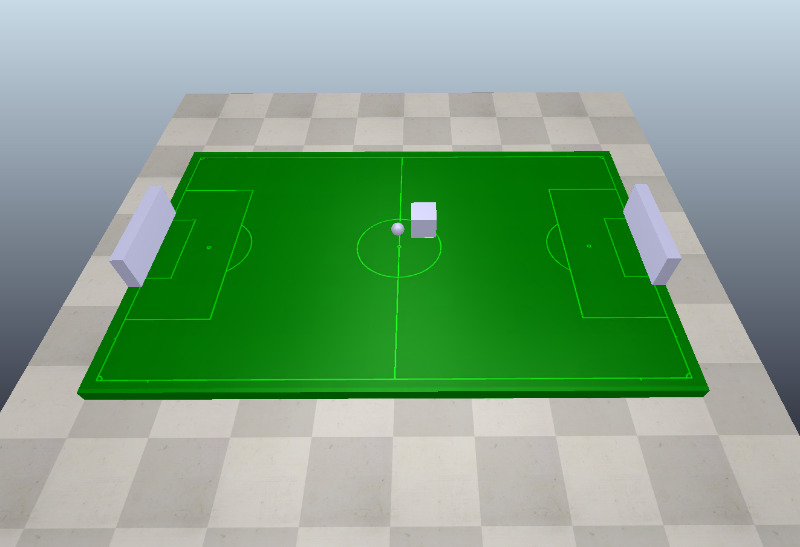
\includegraphics[width=\textwidth]{football_field.png}
  \end{center}
  \caption{足球場景}
  \label{fig:photo}
\end{figure}
